\begin{figure*}[t]
\centering
\captionsetup{font=small}
\captionsetup[subfigure]{font=small}
\begin{minipage}[b]{0.48\textwidth}
\centering
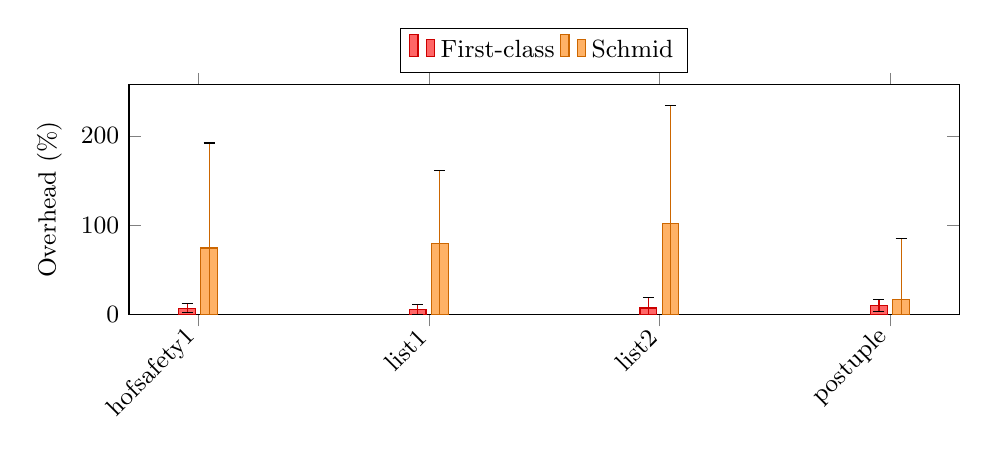
\begin{tikzpicture}
\begin{axis}[
    ybar,
    bar width=6pt,
    width=\textwidth,
    height=4.5cm,
    ylabel={Overhead (\%)}, 
    symbolic x coords={hofsafety1, list1, list2, postuple},
    xtick=data,
    every axis/.style={font=\small},
    x tick label style={rotate=45, anchor=east},
    legend style={at={(0.5,1.05)}, anchor=south, legend columns=2},
    ymin=0,
    enlarge x limits=0.1,
]
\addplot[fill=red!60, draw=red!80!black, error bars/.cd, y dir=both, y explicit]
  coordinates {
    (hofsafety1, 7.1) +- (0, 4.8)
    (list1, 5.8) +- (0, 5.7)
    (list2, 7.3) +- (0, 11.8)
    (postuple, 10.0) +- (0, 6.8)
  };
\addlegendentry{First-class}
\addplot[fill=orange!60, draw=orange!80!black, error bars/.cd, y dir=both, y explicit]
  coordinates {
    (hofsafety1, 74.5) +- (0, 117.6)
    (list1, 79.3) +- (0, 82.1)
    (list2, 102.3) +- (0, 131.6)
    (postuple, 16.9) +- (0, 67.9)
  };
\addlegendentry{Schmid}
\end{axis}
\end{tikzpicture}
\subcaption{vs.\ Schmid}
\label{fig:bench-overhead-schmid}
\end{minipage}
\hspace{0.01\textwidth}
\begin{minipage}[b]{0.48\textwidth}
\centering
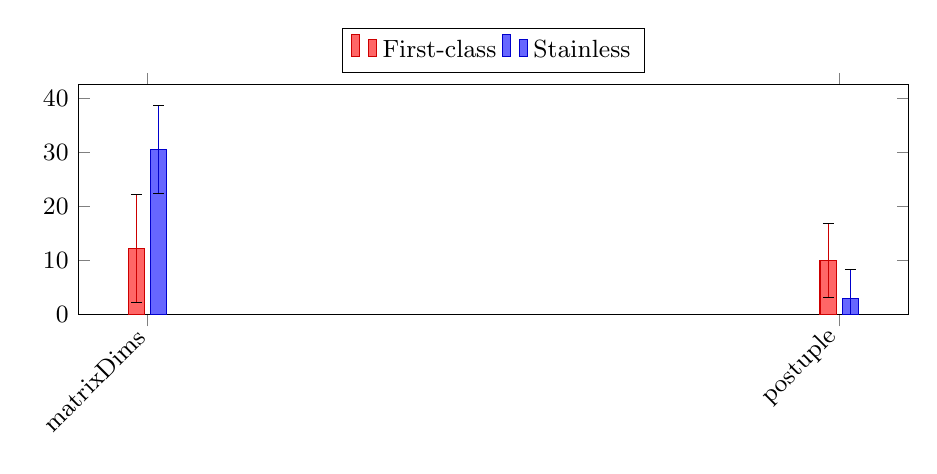
\begin{tikzpicture}
\begin{axis}[
    ybar,
    bar width=6pt,
    width=\textwidth,
    height=4.5cm,
    ylabel={},
    symbolic x coords={matrixDims, postuple},
    xtick=data,
    every axis/.style={font=\small},
    x tick label style={rotate=45, anchor=east},
    legend style={at={(0.5,1.05)}, anchor=south, legend columns=2},
    ymin=0,
    enlarge x limits=0.1,
]
\addplot[fill=red!60, draw=red!80!black, error bars/.cd, y dir=both, y explicit]
  coordinates {
    (matrixDims, 12.2) +- (0, 10.0)
    (postuple, 10.0) +- (0, 6.8)
  };
\addlegendentry{First-class}
\addplot[fill=blue!60, draw=blue!80!black, error bars/.cd, y dir=both, y explicit]
  coordinates {
    (matrixDims, 30.6) +- (0, 8.1)
    (postuple, 3.0) +- (0, 5.3)
  };
\addlegendentry{Stainless}
\end{axis}
\end{tikzpicture}
\subcaption{vs.\ Stainless (note to reviewers: we expect more benchmarks to be added before publication)}
\label{fig:bench-overhead-stainless}
\end{minipage}
\caption{Relative compilation time overhead (\%) compared to the respective unchecked baseline. Error bars show the 95\% confidence interval.}
\label{fig:bench-overhead}
\end{figure*}